% https://www.overleaf.com/project/63bd2ae4eaaeb046af8512b5

% This must be in the first 5 lines to tell arXiv to use pdfLaTeX, which is strongly recommended.
\pdfoutput=1
% In particular, the hyperref package requires pdfLaTeX in order to break URLs across lines.

\documentclass[11pt]{article}

% Remove the "guidelines" option to generate the final version.
\usepackage[guidelines]{nlpreport} % show guidelines
%\usepackage[]{nlpreport} % hide guidelines


% Standard package includes
\usepackage{times}
\usepackage{latexsym}

% For proper rendering and hyphenation of words containing Latin characters (including in bib files)
\usepackage[T1]{fontenc}
% For Vietnamese characters
% \usepackage[T5]{fontenc}
% See https://www.latex-project.org/help/documentation/encguide.pdf for other character sets

% This assumes your files are encoded as UTF8
\usepackage[utf8]{inputenc}

% This is not strictly necessary, and may be commented out,
% but it will improve the layout of the manuscript,
% and will typically save some space.
\usepackage{microtype}
\usepackage{graphicx}
\usepackage{hyperref}
\usepackage{amsmath}
\usepackage{mathtools}
\usepackage{multirow}
\usepackage{listings}
\usepackage{xcolor}
\usepackage{booktabs} % for tables


\usepackage{subfigure}



% THE pdfinfo Title AND Author ARE NOT NECESSARY, THEY ARE METADATA FOR THE FINAL PDF FILE
\hypersetup{pdfinfo={
Title={Assignment 2},
Author={
    Daniel Bernardi,
    Daniele Santini,
    Hiari Pizzini Cavagna
    \&
    Muhammad Saleem Ghulam
}
}}
%\setcounter{secnumdepth}{0}  
 \begin{document}
%
\title{Assignment 2\\
\explanation{\rm Substitute the $\uparrow$ title $\uparrow$ with your project's title, or with Assignment 1 / 2\\ \smallskip}
% subtitle:
\large \explanation{\rm $\downarrow$ Keep only one of the following three  labels  / leave empty for assignments: $\downarrow$\\}
NLP Course Project
}
\author{
    Daniel Bernardi,
    Daniele Santini,
    Hiari Pizzini Cavagna
    \and
    Muhammad Saleem Ghulam\\
Master's Degree in Artificial Intelligence, University of Bologna\\
\{ daniel.bernardi, daniele.santini2, hiari.pizzinicavagna, muhammad.ghulam \}@studio.unibo.it
}
\maketitle


\attention{DO NOT MODIFY THIS TEMPLATE - EXCEPT, OF COURSE FOR TITLE, SUBTITLE AND AUTHORS.\\ IN THE FINAL VERSION, IN THE \LaTeX\ SOURCE REMOVE THE \texttt{guidelines} OPTION FROM  \texttt{$\backslash$usepackage[guidelines]\{nlpreport\}}.
}

\begin{abstract}
%\begin{quote}

\explanation{
The abstract is very brief summary of your report. Try to keep it no longer than 15-20 lines at most. Write your objective, your approach, and your main observations (what are the findings that make this report worthwhile reading?)}

Comparative analysis of Neural-Network based implementations of text generation: combining Transformer based architectures for history-aware question answering.

%\end{quote}
\end{abstract}

\attention{\textcolor{red}{NOTICE: THIS REPORT'S LENGTH MUST RESPECT THE FOLLOWING PAGE LIMITS: \begin{itemize}
    \item ASSIGNMENT: \textbf{2 PAGES} 
    \item NLP PROJECT OR PROJECT WORK: \textbf{8 PAGES}
    \item COMBINED NLP PROJECT + PW: \textbf{12 PAGES}
\end{itemize}  PLUS LINKS, REFERENCES AND APPENDICES.\\ 
THIS MEANS THAT YOU CANNOT FILL ALL SECTIONS TO MAXIMUM LENGTH. IT ALSO MEANS THAT, QUITE POSSIBLY, YOU WILL HAVE TO LEAVE OUT OF THE REPORT PART OF THE WORK YOU HAVE DONE OR OBSERVATIONS YOU HAVE. THIS IS NORMAL: THE REPORT SHOULD EMPHASIZE WHAT IS MOST SIGNIFICANT, NOTEWORTHY, AND REFER TO THE NOTEBOOK FOR ANYTHING ELSE.\\ 
FOR ANY OTHER ASPECT OF YOUR WORK THAT YOU WOULD LIKE TO EMPHASIZE BUT CANNOT EXPLAIN HERE FOR LACK OF SPACE, FEEL FREE TO ADD COMMENTS IN THE NOTEBOOK.\\ 
INTERESTING TEXT EXAMPLES THAT EXCEED THE MAXIMUM LENGTH OF THE REPORT CAN BE PLACED IN A DEDICATED APPENDIX AFTER THE REFERENCES.}}


\section{Introduction}
\label{sec:introduction}
\attention{MAX 1 COLUMN FOR ASSIGNMENT REPORTS / 2 COLUMNS FOR PROJECT OR PW / 3 FOR COMBINED REPORTS.}

\explanation{
The Introduction is an executive summary, which you can think of as an extended abstract.  Start by writing a brief description of the problem you are tackling and why it is important. (Skip it if this is an assignment report).} 

\explanation{Then give a short overview of known/standard/possible approaches to that problems, if any, and what are their advantages/limitations.} 

\explanation{After that, discuss your approach, and motivate why you follow that approach. If you are drawing inspiration from an existing model, study, paper, textbook example, challenge, \dots, be sure to add all the necessary references~\cite{DBLP:journals/corr/abs-2204-02311,DBLP:conf/acl/LorenzoMN22,DBLP:conf/clef/AnticiBIIGR21,DBLP:conf/ijcai/NakovCHAEBPSM21,DBLP:conf/naacl/RottgerVHP22,DBLP:journals/toit/LippiT16}.\footnote{\href{https://en.wikipedia.org/wiki/The_Muppet_Show}{Add only what is relevant.}}}

\explanation{Next, give a brief summary of your experimental setup: how many experiments did you run on which dataset. Last, make a list of the main results or take-home lessons from your work.}

\attention{HERE AND EVERYWHERE ELSE: ALWAYS KEEP IN MIND THAT, CRUCIALLY, WHATEVER TEXT/CODE/FIGURES/IDEAS/... YOU TAKE FROM ELSEWHERE MUST BE CLEARLY IDENTIFIED AND PROPERLY REFERENCED IN THE REPORT.}

The goal of this assignment was to perform Part-Of-Speech tagging using neural architectures on the Dependency Treebanks corpus from NLTK.

The necessary tasks included the download, pre-processing, and analysis of the corpus, the dense embedding of the words in the corpora and the comparation of the results of four Neural Network architectures choosen ahead of time:
\begin{itemize}
    \item Bidirectional LSTM layer + Dense layer (baseline)
    \item Bidirectional GRU layer + Dense layer
    \item 2x Bidirectional LSTM layer + 1x Dense layer
    \item 1x Bidirectional LSTM layer + 2x Dense layer
\end{itemize}

The intended evaluation metric on the test set is F1-Macro, without considering punctuation classes. 

\explanation{
\section{Background}
\label{sec:background}
}
\attention{MAX 2 COLUMNS (3 FOR COMBINED REPORTS). DO NOT INCLUDE SECTION IF NO BACKGROUND NECESSARY. OMIT SECTION IN ASSIGNMENT REPORTS.}

\explanation{The Background section is where you briefly provide whatever background information on the domain or challenge you're addressing and/or on the techniques/approaches you're using, that (1) you think is necessary for the reader to understand your work and design choices, and (2) is not something that has been explained to you during the NLP course (to be clear: do NOT repeat explanations of things seen in class, we already know that stuff). If you adapt paragraphs from articles, books, online resources, etc: be sure to clarify which parts are yours and which ones aren't.}

\section{System description}
\label{sec:system}
\attention{MAX 1 COLUMN FOR ASSIGNMENT REPORTS / 4 COLUMNS FOR PROJECT OR PW / 6 FOR COMBINED REPORTS.}

\explanation{
Describe the system or systems you have implemented (architectures, pipelines, etc), and used to run your experiments. If you reuse parts of code written by others, be sure to make very clear your original contribution in terms of
\begin{itemize}
    \item architecture: is the architecture your design or did you take it from somewhere else
    \item coding: which parts of code are original or heavily adapted? adapted from existing sources? taken from external sources with minimal adaptations?
\end{itemize}
It is a good idea to add figures to illustrate your pipeline and/or architecture(s)
(see Figure~\ref{fig:architecture})
%
\begin{figure*}
    \centering
    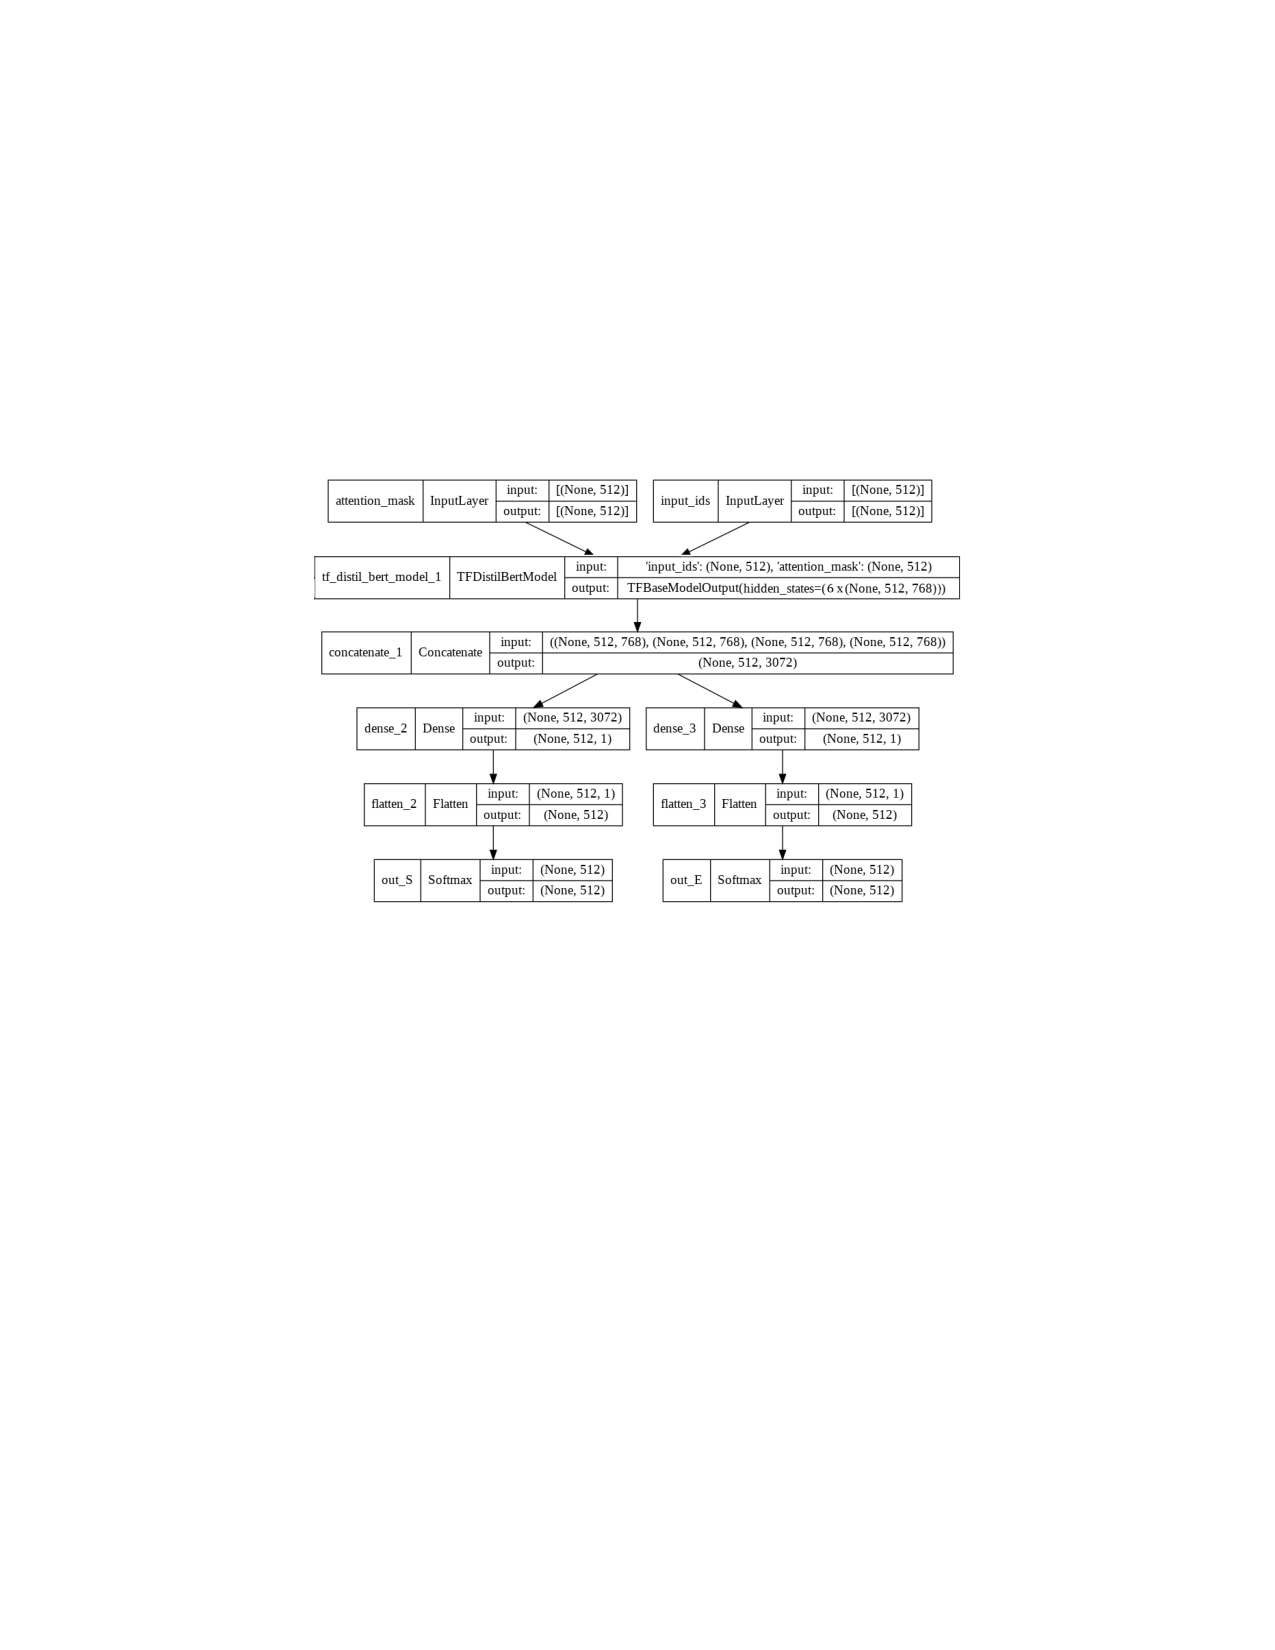
\includegraphics[width=\textwidth]{img/architecture.pdf}
    \caption{Model architecture}
    \label{fig:architecture}
\end{figure*}
}

The corpus download is implemented in plain Python.
Since the corpus files are numbered and the train-val-test split is done before the data loading by selecting a range of files, we have implemented a function (called loadCorpus) which takes in input the range of files to open and loads these as a Pandas DataFrame.

The Exploratory Data Analysis and data pre-processing are implemented using Pandas and Matplotlib.
%We pre-processed the data using Pandas (in particular, we implemented the function cleanCorpus to remove the punctuation classes).

As per instructions, the word embedding was done using the GloVe dense embedding \cite{pennington-etal-2014-glove}.
This was implemented using the glove-wiki-gigaword-200 embedding model\textsuperscript{~\ref{sec:links}} from the gensim library \cite{rehurek_lrec} and using it inside a Tokenizer layer that was used ase the first layer in our Tensorflow neural network.
The Out-Of-Vocabulary words were handled by adding a random embedding vector to the embedding matrix.

Using Python, Numpy and Tensorflow interfaces we made sure to make our code reproducible, then we proceeded to implement the four neural network architectures with Tensorflow.
%For the model architectures, see Figure~\ref{fig:model_architecture}.

% \begin{figure*}
%     \centering
%     %\subfigure[]{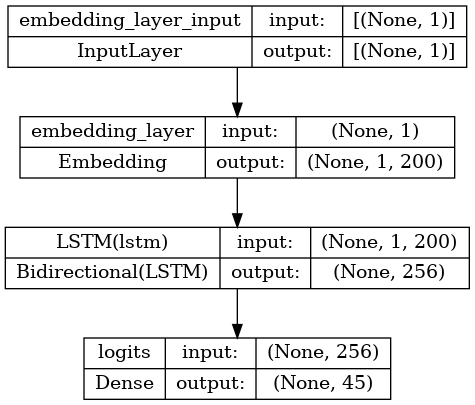
\includegraphics[width=\columnwidth]{base_model.png}}
%     \subfigure[]{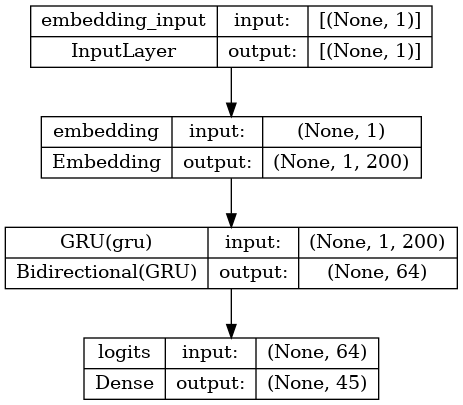
\includegraphics[width=0.32\textwidth]{gru_model.png}}
%     \subfigure[]{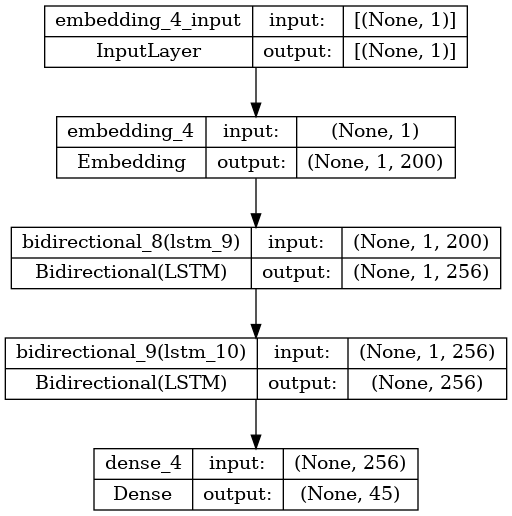
\includegraphics[width=0.32\textwidth]{x2lstm_model.png}}
%     \subfigure[]{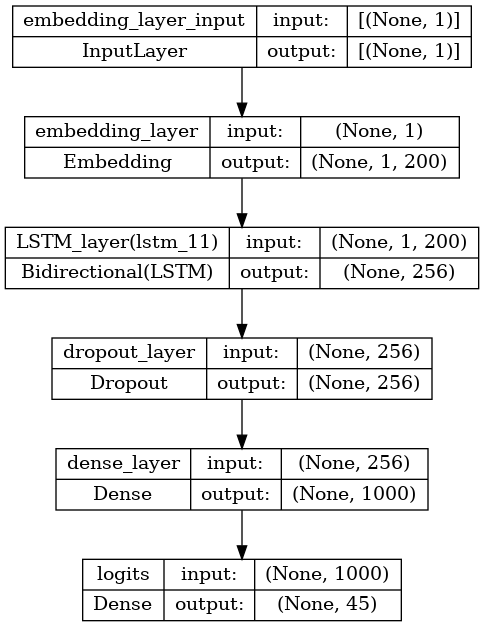
\includegraphics[width=0.32\textwidth]{lstm_dense_model.png}}
%     \caption{Model architectures: (a) LSTM (b) GRU (c) 2xLSTM (d) LSTM+Dense}
%     \label{fig:model_architecture}
% \end{figure*}

\section{Data}
\label{sec:data}
\attention{MAX 2 COLUMNS / 3 FOR COMBINED REPORTS. OMIT SECTION IN ASSIGNMENT REPORTS.}

\explanation{Provide a brief description of your data including some statistics and pointers (references to articles/URLs) to be used to obtain the data. Describe any pre-processing work you did. Links to datasets must be placed later in Section~\ref{sec:links}.}

The corpus contained training, validation and test data.
As mentioned above, it was divided in 200 numbered files and the train-val-test split is done before the data loading by selecting a range of files.

Based on the information available on punctuation\textsuperscript{~\ref{sec:links}}, we have identified these punctuation classes: \verb|``|,  \verb|’’|,  \verb|-LRB-|,  \verb|-RRB-|, 
 \verb|,|,  \verb|.|,  \verb|:|,  \verb|HYPH|,  \verb|\#|,  \verb|\$|, 
 \verb|SYM|,  \verb|''|.
%The distribution of these classes among all classes can be observed in Figure~\ref{fig:classes_with_punct}
The distribution of these classes among all classes can be observed in the Python notebook.

\begin{table*}[!t]
\begin{tabular}{l|l|l|l|l|l|l|l}
\multicolumn{1}{c|}{\textbf{Architecture}} & \textbf{Units} & \textbf{Dropout} & \textbf{Activation} & \textbf{LR} & \textbf{Epochs} & \textbf{Acc.} & \multicolumn{1}{c}{\textbf{F1 Val.}} \\ \hline
Bi-LSTM + Dense		& 32		& 0		& tanh		& 28e-4	& 9 	& 0.885	& 0.707	\\
Bi-GRU + Dense		& 112		& 0.05	& tanh		& 64e-5	& 17	& 0.891	& 0.701	\\
Two Bi-LSTM + Dense	& 128+112	& 0+0.2	& tanh+relu	& 14e-4	& 7		& 0.890	& 0.708	\\
Bi-LSTM + Two Dense	& 112+64    & 0		& relu+tanh	& 12e-4	& 6		& 0.885	& 0.716
\end{tabular}
\caption{Results obtained using Keras Tuner for every different architecture}
\label{table:tuner}
\end{table*}



\section{Experimental setup and results}
\label{sec:results}
\attention{MAX 1 COLUMN FOR ASSIGNMENT REPORTS / 3 COLUMNS FOR PROJECT OR PW / 5 FOR COMBINED REPORTS.}

\explanation{
Describe how you set up your experiments: which architectures/configurations you used, which hyper-parameters and what methods used to set them, which optimizers, metrics, etc.
\\
Then, \textbf{use tables} to summarize your your findings (numerical results) in validation and test. If you don't have experience with tables in \LaTeX, you might want to use \href{https://www.tablesgenerator.com/}{\LaTeX table generator} to quickly create a table template.
}

We first experimented manually tuning the hyper-parameters for these four models.

Then we calibrated the configurations for the four different architectures using 
Keras Tuner\textsuperscript{~\ref{sec:links}}. The hyper-parameters considered and their range (min, max) were: the number of units (16, 256), the activation functions (relu, tanh), dropout (0, 0.2) and learning rate (1e-4, 1e-2), with Adam as optimizer. 
The chosen tuner algorithm was Hyperband \cite{arxiv.1603.06560}, that allows to quickly converge on a high-performing model, comparing possible combinations through a "championship style" bracket. The algorithm used accuracy to determine the best model, training at most for 30 epochs, using the Early Stopping callback with a min. value of 15e-4 to increase the performances. 
The results obtained and the F1-score calculated are showed in the Table \ref{table:tuner}. The F1-score is macro-averaged, calculated excluding all the punctuation classes.  
In the end, the F1-score on the test set has been calculated, both best models had a better score compared with the validation score. 

\begin{table}[!h]
\begin{tabular}{l|l|l}
\multicolumn{1}{c|}{\textbf{Model}}       & \textbf{F1 Val.} & \multicolumn{1}{c}{\textbf{F1 Test}} \\ \hline
2xBi-LSTM + Dense	& 0.708		& 0.782	\\
Bi-LSTM + 2xDense	& 0.716		& 0.793
\end{tabular}
\end{table}

\section{Discussion}
\label{sec:discussion}
\attention{MAX 1.5 COLUMNS FOR ASSIGNMENT REPORTS / 3 COLUMNS FOR PROJECT / 4 FOR COMBINED REPORTS. ADDITIONAL EXAMPLES COULD BE PLACED IN AN APPENDIX AFTER THE REFERENCES IF THEY DO NOT FIT HERE.}


\explanation{
Here you should make your analysis of the results you obtained in your experiments. Your discussion should be structured in two parts: 
\begin{itemize}
    \item discussion of quantitative results (based on the metrics you have identified earlier; compare with baselines);
    \item error analysis: show some examples of odd/wrong/unwanted  outputs; reason about why you are getting those results, elaborate on what could/should be changed in future developments of this work.
\end{itemize}
}

All the models ended up with a F1-score result on the test set around 0.8, good but not perfect.

Since Gated Recurrent Units are less complex than Long Short Term Memory units we weren't surprised to see that the GRU model didn't outperform the baseline LSTM model.

During the initial manual phase we started with a high number of units in the first Dense layer of the last model and noticed that it was particularly susceptible to over-fitting. This problem was addressed and solved by using dropout and early stopping. KerasTuner then demonstrated that a better result could be obtained simply reducing the number of units in the dense layer while keeping early stopping. The optimized hyper-parameters also changed the learning rate and the activation functions, which could have an impact.

As we expected the best performing architectures were the last two, however they didn't substantially outperform the baseline, even after tuning the hyper-parameters with Keras Tuner.

\section{Conclusion}
\label{sec:conclusion}
\attention{MAX 1 COLUMN.}

\explanation{
In one or two paragraphs, recap your work and main results.
What did you observe? 
Did all go according to expectations? 
Was there anything surprising or worthwhile mentioning?
After that, discuss the main limitations of the solution you have implemented, and indicate promising directions for future improvement.
}

Since this problem relies heavily on identifying the relationship between the elements in the string, a possible way to improve the output would be to use attention-based architectures, such as transformer-derived techniques like BERT. Recurrent architectures like LSTM and GRU are partially able to learn these patterns but attention based architectures are precisely designed to exploit these relationships.

\section{Links to external resources}
\label{sec:links}
\attention{THIS SECTION IS OPTIONAL}
\explanation{
Insert here:
\begin{itemize}
    \item a link to your GitHub or any other public repo where one can find your code (only if you did not submit your code on Virtuale); 
    \item a link to your dataset (only for non-standard projects or project works).
\end{itemize}
}

\begin{itemize}
    \item \href{https://raw.githubusercontent.com/nltk/nltk_data/gh-pages/packages/corpora/dependency_treebank.zip}{Corpus}
    \item \href{https://en.wikipedia.org/wiki/English_punctuation}{English punctuation on Wikipedia}
    \item \href{https://universaldependencies.org/docs/en/pos/all.html#al-en-pos/PUNCT}{PUNCT POS tags on Universal Dependencies}
    %\item \href{https://nlp.stanford.edu/projects/glove/}{GloVe}
    \item \href{https://radimrehurek.com/gensim/auto_examples/index.html}{gensim library docs}
    \item \href{https://github.com/RaRe-Technologies/gensim-data#models}{gensim available models}
    \item \href{https://keras.io/api/keras_tuner/}{KerasTuner API - Keras}
    \item \href{https://www.tensorflow.org/tutorials/keras/keras_tuner}{Keras Tuner - Tensorflow}
    \item \href{https://github.com/Danysan1/ai-unibo-nlp-project}{Our GitHub repository}
\end{itemize}
\attention{DO NOT INSERT CODE IN THIS REPORT}



%\bibliography{nlpreport.bib}
\bibliography{nlpreport, main}

% \begin{figure*}
%     \centering
%     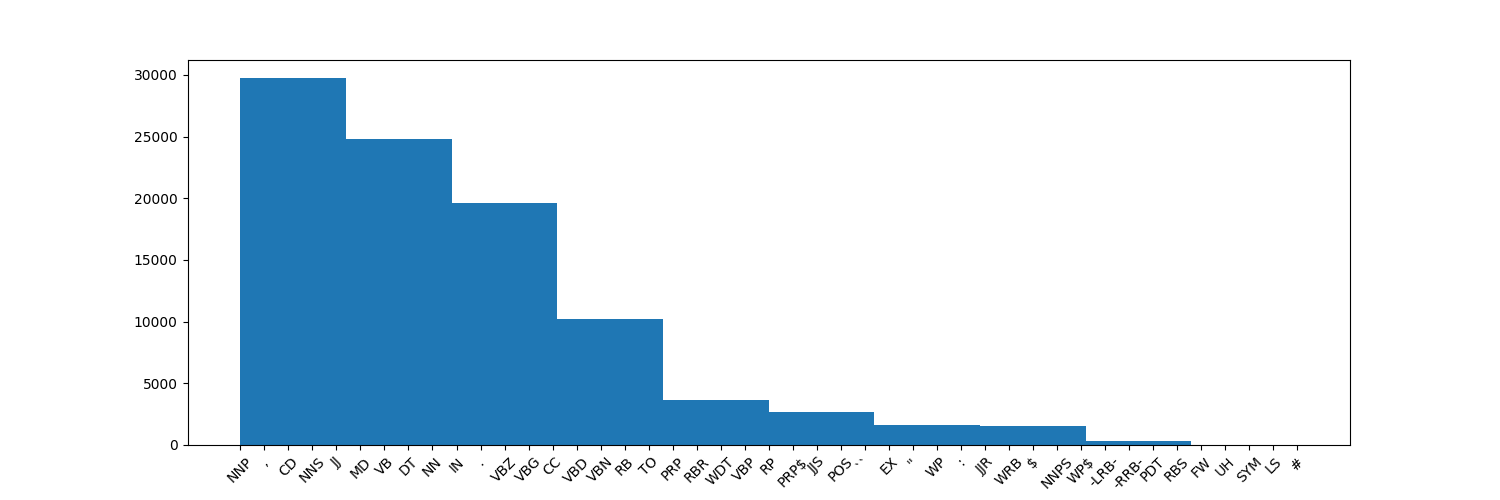
\includegraphics[width=\textwidth]{classes_with_punctuation.png}
%     \caption{Class distribution (including punctuation classes)}
%     \label{fig:classes_with_punct}
% \end{figure*}

\end{document}